\section{Experiments}
    
\label{sec:experiments}
\subsection{Experimental Setup}
    
We evaluate \name{} in agent distillation. We supervise thoughts and actions from the trajectories and fine-tune the student models using LoRA. The specific training configurations are rank $32$, learning rate $2\times10^{-4}$, and $\alpha = 64$. Prior traffic-analysis systems have reported identification precision above $70\%$~\cite{chiang2024chatbot, liu2026embarrassingly}. We therefore adopt a more conservative $50\%$ precision setting to avoid missing potential distillation traces, with $|\mathcal{S}|=100$ suspicious trajectories and $|\mathcal{D}_c|=50$ trajectories used for distillation. Appendix~\ref{sec:experimental-details} provides the remaining experimental details, including hyperparameter selection and baselines. Our experiments assess watermark effectiveness, harmlessness, robustness against adversarial processing.

\partitle{Datasets and Models} Our evaluation spans three datasets: BFCL~\cite{patil2025berkeley}, SWE-bench~\cite{jimenez2024swe}, and Telecom (a service-tool domain from the Tau2 benchmark\footnote{\url{https://github.com/sierra-research/tau2-bench}}). GPT-OSS-120B~\cite{agarwal2025gpt} and Kimi-K2.5~\cite{team2026kimi} serve as teacher agents ($\mathcal{M}_t$), with Qwen3-8B acting as both the candidate scorer ($\mathcal{M}_q$) and safety model ($\mathcal{M}_{\mathtt{safe}}$). For distillation, we fine-tune four student models ($\mathcal{M}_s$): Mistral-Small-3.1-24B~\cite{liu2026ministral}, Qwen3-14B~\cite{yang2025qwen3}, Qwen3-32B~\cite{yang2025qwen3}, and GLM-4.7-Flash~\cite{glm2024chatglm}.

\partitle{Evaluation metrics} For detection, we report strict fullhit rates $(R_\tau^{\mathtt{real}},R_\tau^{\mathtt{fake}})$ on real and fake probes, alongside the one-sided $p$-value. A successful detection requires $p<0.05$ and a real-fake mean fullhit gap $\ge 0.05$. For trace-level attribution, we measure $\operatorname{\mathtt{Precision}}@K$ of top-$K$ trajectories belonging to the distillation subset $\mathcal{D}_c$. For harmlessness, we compare task accuracy ($\mathtt{Acc}$) and mean interaction steps ($L$) between control and watermarked agents.

\subsection{Effectiveness}

\label{sec:detection-effectiveness}

\begin{table*}[!t]
\centering
\setlength{\tabcolsep}{3.5pt}
\caption{True-positive results. Cards is the number of cards; hit-rate cells report hits / probes (rate). $w/\ell$ gives card-level real / fake wins. The `Sig' column indicates statistical significance: {\color{green}$\checkmark$} denotes $p < 0.05$, indicating a statistically significant change, whereas {\color{red}$\times$} denotes $p \ge 0.05$.}

\label{tab:true-positive}
\scriptsize
\begin{tabular}{l l c l | c c c c c}
\noalign{\hrule height 1.5pt}
\multirow{2}{*}{\textbf{Teacher Agent$\mathcal{M}_t$}} & \multirow{2}{*}{\textbf{Dataset}} & \multirow{2}{*}{\textbf{Cards}} & \multirow{2}{*}{\textbf{Student Model $\mathcal{M}_s$}} & \multicolumn{5}{c}{\textbf{Detection Results}} \\
\cline{5-9}
& & & & \textbf{$R^{\mathtt{real}}$ (\%)} & \textbf{$R^{\mathtt{fake}}$ (\%)} & \textbf{$w/\ell$} & \textbf{$p$-value} & \textbf{Sig.} \\
\hline
\multirow{4}{*}{GPT-OSS-120B} & \multirow{4}{*}{BFCL} & \multirow{4}{*}{118} & Mistral-24B & \tableRate{93}{182}{51.1} & \tableRate{59}{182}{32.4} & 25 / 1 & \tablePval{4.0}{-7} & {\color{green}\checkmark} \\
& & & GLM-4.7-Flash & \tableRate{108}{182}{59.3} & \tableRate{80}{182}{44.0} & 19 / 1 & \tablePval{2.0}{-5} & {\color{green}\checkmark} \\
& & & Qwen3-14B & \tableRate{44}{182}{24.2} & \tableRate{28}{182}{15.4} & 20 / 4 & \tablePval{7.7}{-4} & {\color{green}\checkmark} \\
& & & Qwen3-32B & \tableRate{89}{182}{48.9} & \tableRate{58}{182}{31.9} & 30 / 9 & \tablePval{5.3}{-4} & {\color{green}\checkmark} \\
\hline
\multirow{4}{*}{Kimi-K2.5} & \multirow{4}{*}{BFCL} & \multirow{4}{*}{145} & Mistral-24B & \tableRate{175}{379}{46.2} & \tableRate{105}{379}{27.7} & 45 / 10 & \tablePval{1.0}{-6} & {\color{green}\checkmark} \\
& & & GLM-4.7-Flash & \tableRate{155}{379}{40.9} & \tableRate{69}{379}{18.2} & 47 / 4 & \tablePval{1.2}{-10} & {\color{green}\checkmark} \\
& & & Qwen3-14B & \tableRate{102}{379}{26.9} & \tableRate{26}{379}{6.9} & 46 / 4 & \tablePval{2.2}{-10} & {\color{green}\checkmark} \\
& & & Qwen3-32B & \tableRate{82}{379}{21.6} & \tableRate{18}{379}{4.7} & 39 / 5 & \tablePval{7.0}{-8} & {\color{green}\checkmark} \\
\noalign{\hrule height 1.5pt}
\end{tabular}
\end{table*}


In this section, all student models are trained on the original  dataset $\mathcal{D}_c$. We test our scheme on distilled and clean models via separate true positive and false positive experiments. We also evaluate the performance of existing agent watermark baselines under the matched setting. Furthermore, we evaluate \name{}'s trace-level attribution using $\operatorname{\mathtt{Precision}}@K$ in Appendix~\ref{sec:supplementary-effectiveness}. Finally, we measure how identification accuracy affects statistical significance in Appendix~\ref{sec:supplementary-effectiveness}.



\partitle{True positives} We first evaluate whether \name{} can successfully identify student models distilled from watermarked trajectories. Our experiments cover all combinations of 3 datasets (SWE and Telecom are in Appendix~\ref{sec:supplementary-effectiveness}), 2 teacher agents, and 4 student models. In each setting, we compare the hit rates between the real side and the fake side and calculate the $p$-value. The results in the Table~\ref{tab:true-positive} and~\ref{tab:appendix-true-positive} show that \name{} successfully achieves detection in all settings. These results show that \name{} can extract watermark from student models of different architectures.


\partitle{False positives} We evaluate whether \name{} causes false positives on clean models that have not seen watermarked trajectories. As shown in Table~\ref{tab:false-positive} and Table~\ref{tab:appendix-false-positive} in Appendix~\ref{sec:supplementary-effectiveness}, in addition to the four undistilled student models, we also select four base models (DeepSeek-V4-Flash \cite{xu2026deepseek}, MiniMax-M2.5 \cite{chen2026minimax}, Qwen3.5-Flash \cite{yang2025qwen3}, and MiMo-V2.5 \cite{xiao2026mimo}) and build a total of 48 controlled false-positive evaluation settings. The results show that \name{} achieves zero false positives across all 48 settings.

\begin{table*}[!t]
\caption{False-positive results. The `Sig' column indicates statistical significance: {\color{green}$\checkmark$} denotes $p < 0.05$, indicating a statistically significant change, whereas {\color{red}$\times$} denotes $p \ge 0.05$.}
\label{tab:false-positive}
\centering
\setlength{\tabcolsep}{5.3pt}
\scriptsize
\begin{tabular}{l l c l | c c c c c}
\noalign{\hrule height 1.5pt}
\multirow{2}{*}{\textbf{Teacher Agent$\mathcal{M}_t$}} & \multirow{2}{*}{\textbf{Dataset}} & \multirow{2}{*}{\textbf{Cards}} & \multirow{2}{*}{\textbf{Clean Model $\mathcal{M}_c$}} & \multicolumn{5}{c}{\textbf{Detection Results}} \\
\cline{5-9}
& & & & \textbf{$R^{\mathtt{real}}$ (\%)} & \textbf{$R^{\mathtt{fake}}$ (\%)} & \textbf{$w/\ell$} & \textbf{$p$-value} & \textbf{Sig.} \\
\hline
\multirow{8}{*}{GPT-OSS-120B} & \multirow{8}{*}{BFCL} & \multirow{8}{*}{118} & DeepSeek-V4-Flash & \tableRate{10}{182}{5.5} & \tableRate{11}{182}{6.0} & 2 / 3 & \tablePval{8.1}{-1} & {\color{red}$\times$} \\
& & & MiniMax-M2.5 & \tableRate{9}{182}{4.9} & \tableRate{10}{182}{5.5} & 2 / 3 & \tablePval{8.1}{-1} & {\color{red}$\times$} \\
& & & Mistral-24B & \tableRate{9}{182}{4.9} & \tableRate{7}{182}{3.8} & 3 / 2 & \tablePval{5.0}{-1} & {\color{red}$\times$} \\
& & & Qwen3-14B & \tableRate{7}{182}{3.8} & \tableRate{6}{182}{3.3} & 2 / 1 & \tablePval{5.0}{-1} & {\color{red}$\times$} \\
& & & Qwen3-32B & \tableRate{4}{182}{2.2} & \tableRate{4}{182}{2.2} & 2 / 2 & \tablePval{6.9}{-1} & {\color{red}$\times$} \\
& & & Qwen3.5-Flash & \tableRate{8}{182}{4.4} & \tableRate{8}{182}{4.4} & 2 / 1 & \tablePval{5.0}{-1} & {\color{red}$\times$} \\
& & & MiMo-V2.5 & \tableRate{10}{182}{5.5} & \tableRate{11}{182}{6.0} & 2 / 2 & \tablePval{6.9}{-1} & {\color{red}$\times$} \\
& & & GLM-4.7-Flash & \tableRate{5}{182}{2.7} & \tableRate{1}{182}{0.5} & 4 / 0 & \tablePval{6.2}{-2} & {\color{red}$\times$} \\
\hline
\multirow{8}{*}{Kimi-K2.5} & \multirow{8}{*}{BFCL} & \multirow{8}{*}{145} & DeepSeek-V4-Flash & \tableRate{10}{379}{2.6} & \tableRate{9}{379}{2.4} & 5 / 4 & \tablePval{5.0}{-1} & {\color{red}$\times$} \\
& & & MiniMax-M2.5 & \tableRate{6}{379}{1.6} & \tableRate{3}{379}{0.8} & 4 / 2 & \tablePval{3.4}{-1} & {\color{red}$\times$} \\
& & & Mistral-24B & \tableRate{1}{379}{0.3} & \tableRate{3}{379}{0.8} & 1 / 2 & \tablePval{8.8}{-1} & {\color{red}$\times$} \\
& & & Qwen3-14B & \tableRate{1}{379}{0.3} & \tableRate{0}{379}{0.0} & 1 / 0 & \tablePval{5.0}{-1} & {\color{red}$\times$} \\
& & & Qwen3-32B & \tableRate{1}{379}{0.3} & \tableRate{0}{379}{0.0} & 1 / 0 & \tablePval{5.0}{-1} & {\color{red}$\times$} \\
& & & Qwen3.5-Flash & \tableRate{0}{379}{0.0} & \tableRate{0}{379}{0.0} & 0 / 0 & \tablePval{1.0}{0} & {\color{red}$\times$} \\
& & & MiMo-V2.5 & \tableRate{6}{379}{1.6} & \tableRate{6}{379}{1.6} & 4 / 3 & \tablePval{5.0}{-1} & {\color{red}$\times$} \\
& & & GLM-4.7-Flash & \tableRate{2}{379}{0.5} & \tableRate{2}{379}{0.5} & 2 / 1 & \tablePval{5.0}{-1} & {\color{red}$\times$} \\
\noalign{\hrule height 1.5pt}
\end{tabular}
\end{table*}




\begin{table}[!t]
\centering
\caption{Baseline effectiveness. Agentwm is significant at $\geq3/5$ passes; SeqWM at median $p<0.05$.}
\label{tab:baseline-effectiveness}
\scriptsize
\setlength{\tabcolsep}{3pt}
\begin{tabular}{l l | c c | c c}
\noalign{\hrule height 1.5pt}
\multirow{2}{*}{\textbf{Dataset}} & \multirow{2}{*}{\textbf{Student Model $\mathcal{M}_s$}} & \multicolumn{2}{c|}{\textbf{Agentwm}} & \multicolumn{2}{c}{\textbf{SeqWM}} \\
\cline{3-6}
& & \textbf{Passes} & \textbf{Sig.} & \textbf{Median $p$} & \textbf{Sig.} \\
\hline
\multirow{4}{*}{BFCL} & Mistral-24B & 1/5 & {\color{red}$\times$} & 0.6848 & {\color{red}$\times$} \\
& GLM-4.7-Flash & 3/5 & {\color{green}\checkmark} & 0.5130 & {\color{red}$\times$} \\
& Qwen3-14B & 1/5 & {\color{red}$\times$} & 0.4650 & {\color{red}$\times$} \\
& Qwen3-32B & 2/5 & {\color{red}$\times$} & 0.5744 & {\color{red}$\times$} \\
\cline{1-6}
\multirow{4}{*}{SWE-bench} & Mistral-24B & 1/5 & {\color{red}$\times$} & 0.6274 & {\color{red}$\times$} \\
& GLM-4.7-Flash & 3/5 & {\color{green}\checkmark} & 0.5914 & {\color{red}$\times$} \\
& Qwen3-14B & 1/5 & {\color{red}$\times$} & 0.7073 & {\color{red}$\times$} \\
& Qwen3-32B & 0/5 & {\color{red}$\times$} & 0.4895 & {\color{red}$\times$} \\
\noalign{\hrule height 1.5pt}
\end{tabular}
\end{table}

\partitle{Baseline effectiveness} We evaluate the effectiveness of the two baseline schemes under the matched distillation setting and the details about baselines are in Appendix~\ref{sec:experimental-details}. As shown in Table~\ref{tab:baseline-effectiveness}, for Agentwm, only the GLM-4.7-Flash student model meets the passing criterion of $\geq 3/5$ passes, while all other students fail. For Seqwm, the median $p$-values across all tested models are greater than 0.05, failing to successfully detect any distilled models. As expected, baselines fail, because Seqwm is not designed for antidistillation, and Agentwm has weak watermark signals that requires identical teacher and student base models.

\subsection{Harmlessness}
\label{sec:harmlessness}

\partitle{Harmlessness} A reasonable watermark scheme should not noticeably affect the performance of the teacher agent. Therefore, we evaluate impact of \name{} on the teacher agent $\mathcal{M}_t$'s task utility and inference cost. For the four cohorts in BFCL and Telecom, we compare the unwatermarked agent $\mathcal{M}_\mathtt{tc}$ and the watermarked teacher agent $\mathcal{M}_t$ on 200 tasks. We measure the task accuracy difference $\Delta \mathtt{Acc} = \mathbb{E}[\mathtt{Acc}(\mathcal{M}_t) - \mathtt{Acc}(\mathcal{M}_\mathtt{tc})]$ and the expected interaction step difference $\Delta L = \mathbb{E}[L(\mathcal{M}_t) - L(\mathcal{M}_\mathtt{tc})]$. As summarized in Figure~\ref{fig:harmlessness}, embedding the watermark does not cause a drop in overall performance. The task accuracy difference $\Delta \mathtt{Acc}$ ranges only from $-3.0\%$ to $+3.0\%$, indicating that the accuracy loss is acceptable. Meanwhile, the increase in interaction cost is acceptable: the average step count increases from 20.49 to 21.09 steps, and $\Delta L$ ranges from $-1.38$ to $+2.04$ steps.

\begin{figure*}[!t]
\centering
\begin{subfigure}[t]{0.242\textwidth}
\centering
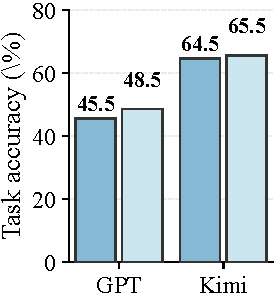
\includegraphics[width=0.82\linewidth]{figure/harmlessness_accuracy_bfcl.pdf}
\caption{BFCL: accuracy}
\end{subfigure}\hfill
\begin{subfigure}[t]{0.242\textwidth}
\centering
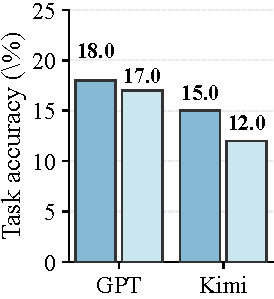
\includegraphics[width=0.82\linewidth]{figure/harmlessness_accuracy_telecom.pdf}
\caption{Telecom: accuracy}
\end{subfigure}\hfill
\begin{subfigure}[t]{0.242\textwidth}
\centering
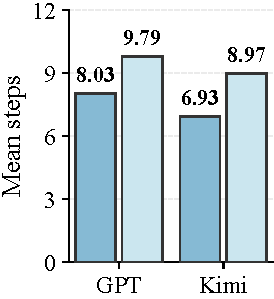
\includegraphics[width=0.82\linewidth]{figure/harmlessness_steps_bfcl.pdf}
\caption{BFCL: steps}
\end{subfigure}\hfill
\begin{subfigure}[t]{0.242\textwidth}
\centering
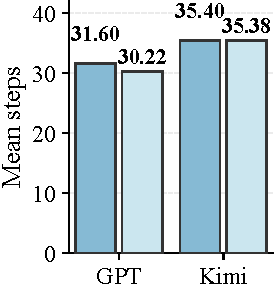
\includegraphics[width=0.82\linewidth]{figure/harmlessness_steps_telecom.pdf}
\caption{Telecom: steps}
\end{subfigure}
\caption{
Harmlessness results. In (a) and (b), the vertical axis reports accuracy; in (c) and (d), it reports the mean number of steps. Colors distinguish \textcolor[HTML]{86BAD4}{$\blacksquare$} unwatermarked and \textcolor[HTML]{CBE6EF}{$\blacksquare$} watermarked runs.
}

\label{fig:harmlessness}
\end{figure*}


\subsection{Robustness}
\label{sec:robustness}

To demonstrate the robustness of our watermark scheme, We evaluate \name{}'s robustness against four common pre-distillation data transformations. These operations include: data flooding, paraphrasing attack, adaptive attack, advanced data flooding and truncation (the last two are in Appendix~\ref{sec:supplementary-robustness}). We evaluate the robustness of Agentwm under data flooding in Appendix~\ref{sec:supplementary-robustness}. We use GPT-OSS-120B as the teacher agent.

\partitle{Data flooding} Before distillation, an attacker may mix the training set with standard clean data to improve distillation performance~\cite{ouyang2022training, mukherjee2023orca}, which will dilutes the watermark signals. To evaluate its impact on our watermark strength, we mix the original watermarked dataset $\mathcal{D}_c$ with clean standard answers. Specifically, in the D1, D5, and D10 settings, we incorporate $1\times$, $5\times$, and $10\times$ the amount of clean data relative to $\mathcal{D}_c$. We evaluate a total of 24 settings across 2 benchmarks (BFCL and SWE-bench), 3 dilution ratios, and 4 student models. As shown in Figure~\ref{fig:data-flooding-robustness}, \name{} successfully detects every setting. Even under the strongest $1{:}10$ dilution ratio, all 8 tested student models remain successfully detected.
\begin{figure*}[!t]
\centering
\begin{subfigure}[t]{\robustnessPanelWidth}
\centering
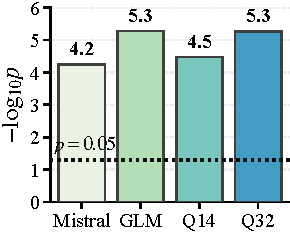
\includegraphics[width=0.72\linewidth]{figure/robustness_data_flooding_bfcl_d1.pdf}
\caption{BFCL: D1}
\end{subfigure}\hfill
\begin{subfigure}[t]{\robustnessPanelWidth}
\centering
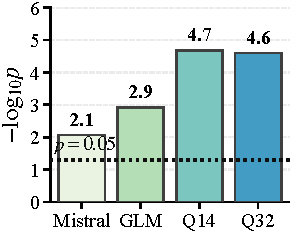
\includegraphics[width=0.72\linewidth]{figure/robustness_data_flooding_bfcl_d5.pdf}
\caption{BFCL: D5}
\end{subfigure}\hfill
\begin{subfigure}[t]{\robustnessPanelWidth}
\centering
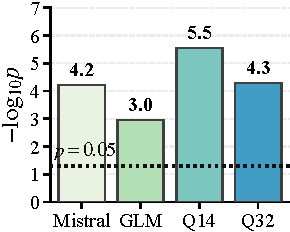
\includegraphics[width=0.72\linewidth]{figure/robustness_data_flooding_bfcl_d10.pdf}
\caption{BFCL: D10}
\end{subfigure}\par
\begin{subfigure}[t]{\robustnessPanelWidth}
\centering
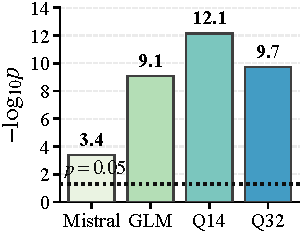
\includegraphics[width=0.72\linewidth]{figure/robustness_data_flooding_swe_bench_d1.pdf}
\caption{SWE-bench: D1}
\end{subfigure}\hfill
\begin{subfigure}[t]{\robustnessPanelWidth}
\centering
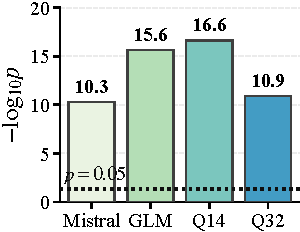
\includegraphics[width=0.72\linewidth]{figure/robustness_data_flooding_swe_bench_d5.pdf}
\caption{SWE-bench: D5}
\end{subfigure}\hfill
\begin{subfigure}[t]{\robustnessPanelWidth}
\centering
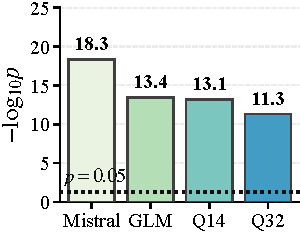
\includegraphics[width=0.72\linewidth]{figure/robustness_data_flooding_swe_bench_d10.pdf}
\caption{SWE-bench: D10}
\end{subfigure}

\caption{Data-flooding robustness. The vertical axis reports $-\log_{10}p$. In (a)--(f), \robustnessModelLegend. The \textcolor[HTML]{8C8C8C}{\hdashrule[0.5ex]{1.2em}{1.2pt}{1pt 1.5pt}} marks $p=0.05$.}

\label{fig:data-flooding-robustness}
\end{figure*}

\begin{table}[!t]
\centering
\caption{Paraphrasing attack robustness.}
\label{tab:semantic-rewriting-robustness}
\scriptsize
\setlength{\tabcolsep}{2pt}
\begin{tabular*}{\linewidth}{@{\extracolsep{\fill}}l l | c c@{}}
\noalign{\hrule height 1.5pt}
\textbf{Dataset} & \textbf{Student Model $\mathcal{M}_s$} & \textbf{$p$-value} & \textbf{Sig.} \\
\hline
\multirow{4}{*}{BFCL} & Mistral-24B & \tablePval{5.7}{-5} & {\color{green}\checkmark} \\
& GLM-4.7-Flash & \tablePval{1.4}{-4} & {\color{green}\checkmark} \\
& Qwen3-14B & \tablePval{3.3}{-3} & {\color{green}\checkmark} \\
& Qwen3-32B & \tablePval{9.8}{-5} & {\color{green}\checkmark} \\
\hline
\multirow{4}{*}{Telecom} & Mistral-24B & \tablePval{3.2}{-2} & {\color{green}\checkmark} \\
& GLM-4.7-Flash & \tablePval{1.4}{-5} & {\color{green}\checkmark} \\
& Qwen3-14B & \tablePval{3.5}{-3} & {\color{green}\checkmark} \\
& Qwen3-32B & \tablePval{4.1}{-3} & {\color{green}\checkmark} \\
\noalign{\hrule height 1.5pt}
\end{tabular*}
\end{table}
\partitle{Paraphrasing attack} An attacker may paraphrase the trajectories, aiming to alter semantic patterns and evade watermark detection while preserving the utility~\cite{krishna2023paraphrasing}. To evaluate the robustness against this rewriting attack, we use DeepSeek-V4-Flash to paraphrase the  $\mathcal{D}_c$. Subsequently, we train 4 student models on these rewritten datasets across the BFCL and Telecom and detect their watermark signals. As reported in Table~\ref{tab:semantic-rewriting-robustness}, \name{} successfully detects the watermark across all 8 settings showing our scheme's robustness under paraphrasing.

\begin{table}[!t]
\centering
\caption{Adaptive attack robustness.}
\label{tab:adaptive-attack}
\scriptsize
\setlength{\tabcolsep}{2pt}
\begin{tabular*}{\linewidth}{@{\extracolsep{\fill}}l l | c c@{}}
\noalign{\hrule height 1.5pt}
\textbf{Dataset} & \textbf{Student Model $\mathcal{M}_s$} & \textbf{$p$-value} & \textbf{Sig.} \\
\hline
\multirow{4}{*}{BFCL} & Mistral-24B & \tablePval{9.2}{-4} & {\color{green}\checkmark} \\
& GLM-4.7-Flash & \tablePval{1.4}{-4} & {\color{green}\checkmark} \\
& Qwen3-14B & \tablePval{9.6}{-3} & {\color{green}\checkmark} \\
& Qwen3-32B & \tablePval{4.1}{-4} & {\color{green}\checkmark} \\
\hline
\multirow{4}{*}{Telecom} & Mistral-24B & \tablePval{2.8}{-8} & {\color{green}\checkmark} \\
& GLM-4.7-Flash & \tablePval{3.7}{-3} & {\color{green}\checkmark} \\
& Qwen3-14B & \tablePval{1.0}{-11} & {\color{green}\checkmark} \\
& Qwen3-32B & \tablePval{5.5}{-12} & {\color{green}\checkmark} \\
\noalign{\hrule height 1.5pt}
\end{tabular*}
\end{table}
\partitle{Adaptive attack} In this section, we consider a stronger attacker who knows that our watermark relies on auxiliary behaviors. To avoid detection, the attacker uses DeepSeek-V4-Flash to clean the collected data by finding and removing suspected auxiliary action while keeping the trajectories useful. Next, we fine-tune student models on this cleaned data and test them on BFCL and Telecom. As shown in Table~\ref{tab:adaptive-attack}, even with this removal, \name{} successfully detects all student models (with the minimal $p$-value of $9.6\times10^{-3}$). This shows that our watermark is highly robust, even when an attacker actively tries to move the signals.


